
%version 2: \usepackage{hyperref}


%%%%%%%%%%%%%%%%%%%%%%%%%%%%%%%%%%%%%%%%%%%%%%%%%%%%%%%%%%%%%%%%%%%%%%%%
%Para las ecuaciones siempre es Ec.(n).
%Para las figuras siempre es Fig.n, incluso en el caption de la figura. Tambien las Tablas
%Para las referencias es [n]
%%%%%%%%%%%%%%%%%%%%%%%%%%%%%%%%%%%%%%%%%%%%%%%%%%%%%%%%%%%%%%%%%%%%%%%%

\documentclass[
reprint,
%notitlepage,
%superscriptaddress,
%groupedaddress,
%unsortedaddress,
%runinaddress,
%frontmatterverbose, 
%preprint,
%showpacs,preprintnumbers,
%nofootinbib,
%nobibnotes,
%bibnotes,
%11 pt,
amsmath,
amssymb,
%aps,
%pra,
prb,
%rmp,
%tightenlines %esto hizo el milagro de sacar los espacios en blancos estocásticos (?)
%prstab,
%prstper,
%floatfix,\textbf{}
]{revtex4-1} %Instalar primero para usarlo. Paquete malo.

%\documentclass[onecolumn, aps, amsmath,amssymb ]{article}
\usepackage{lipsum}  
\usepackage{graphicx}% Include figure files
\usepackage{subfig}
\usepackage{braket}
\usepackage{comment} %comment large chunks of text
\usepackage{dcolumn}% Align table columns on decimal point
\usepackage{bm}% bold math
%\usepackage{hyperref}% add hypertext capabilities
\usepackage[mathlines]{lineno}% Enable numbering of text and display math
%\linenumbers\relax % Commence numbering lines
\usepackage{mathtools} %% Para el supraíndice

\usepackage[nice]{nicefrac}

%%%%%%%El Señor Español%%%%%%%%%%%%%%%%%%%%%%%%%%%
\usepackage[utf8]{inputenc} %acento
\usepackage[
spanish, %El lenguaje.
es-tabla, %La tabla y no cuadro.
activeacute, %El acento.
es-nodecimaldot %Punto y no coma con separador de números
]{babel}
\usepackage{microtype} %para hacerlo más bonito :33 como vos (?) 
%%%%%%%%%%%%%%%%%%%%%%%%%%%%%%%%%%%%%%%%%%%%%%%%%%%
%%%%%%%%% Para que las imágenes se queden dónde las quiero (?
\usepackage{float}
%%%%%%%%%%
\usepackage{enumitem}
\usepackage{hyperref} % Para usar \url

%%%%%%%%Cambia a Fig de Figure%%%%%%%%%%
\makeatletter
\renewcommand{\fnum@figure}{Fig. \thefigure} 
\makeatother
%%%%%%%%%%%%%%%%%%%%%%%%%%%%%%%%%%%%%%%%
\raggedbottom

\usepackage{multirow}
\begin{document}

\title{Práctica 5: Keras}
\author{Evelyn G. Coronel}

\affiliation{Redes Neuronales y Aprendizaje Profundo para Visión Artificial\\ Instituto Balseiro\\}

\date[]{\lowercase{\today}} 

\maketitle

\section*{Ejercicio 3}

    En este ejercicio se utilizó la red \verb|MobileNet| \cite{mobilenet} seguida de una capa densa de 10 valores de salida. Se utilizó está red por ser una red convolucional profunda con una arquitectura liviana.  Esta red ya está implementa en \verb|Keras| y tiene la opción de inicializarla con pesos ya entrenados con el conjunto de datos \emph{imagenet}. Este conjunto consiste en imágenes clasificadas en 1000 categorías. En este ejercicio se estudió la posibilidad de usar los pesos pre-entrenados para clasificar la base de datos del CIFAR-10.

    La red \verb|MobileNet| alcanza un precisión del $70.6\%$ con \emph{imagenet}\cite{mobilenet}, es de esperar que la red obtenga una precisión similar con el CIFAR-10. En las Figs.\ref{fig:ejer3_acc} y \ref{fig:ejer3_loss} se muestran las curvas de entrenamiento (E) y validación  (V) para distintas condiciones de entrenamiento. 

    Primeramente, utilizando la red \verb|MobileNet| con pesos aleatorio, luego se entrenó el modelo implementado durante 60 épocas mediante el optimizador Adam con una tasa de entrenamiento de $10^{-4}$, todo esto con la función de costo del \verb|CategoricalCrossentropy| y la métrica \verb|CategoricalAccuracy|. Para este caso la red llegó a una precisión de  $35.4\%$ después de 60 épocas, esto es de esperarse ya que la red empieza sin noción de los pesos en las capas convolucionales.
    \begin{figure}[H]
        \begin{small}
            \begin{center}
                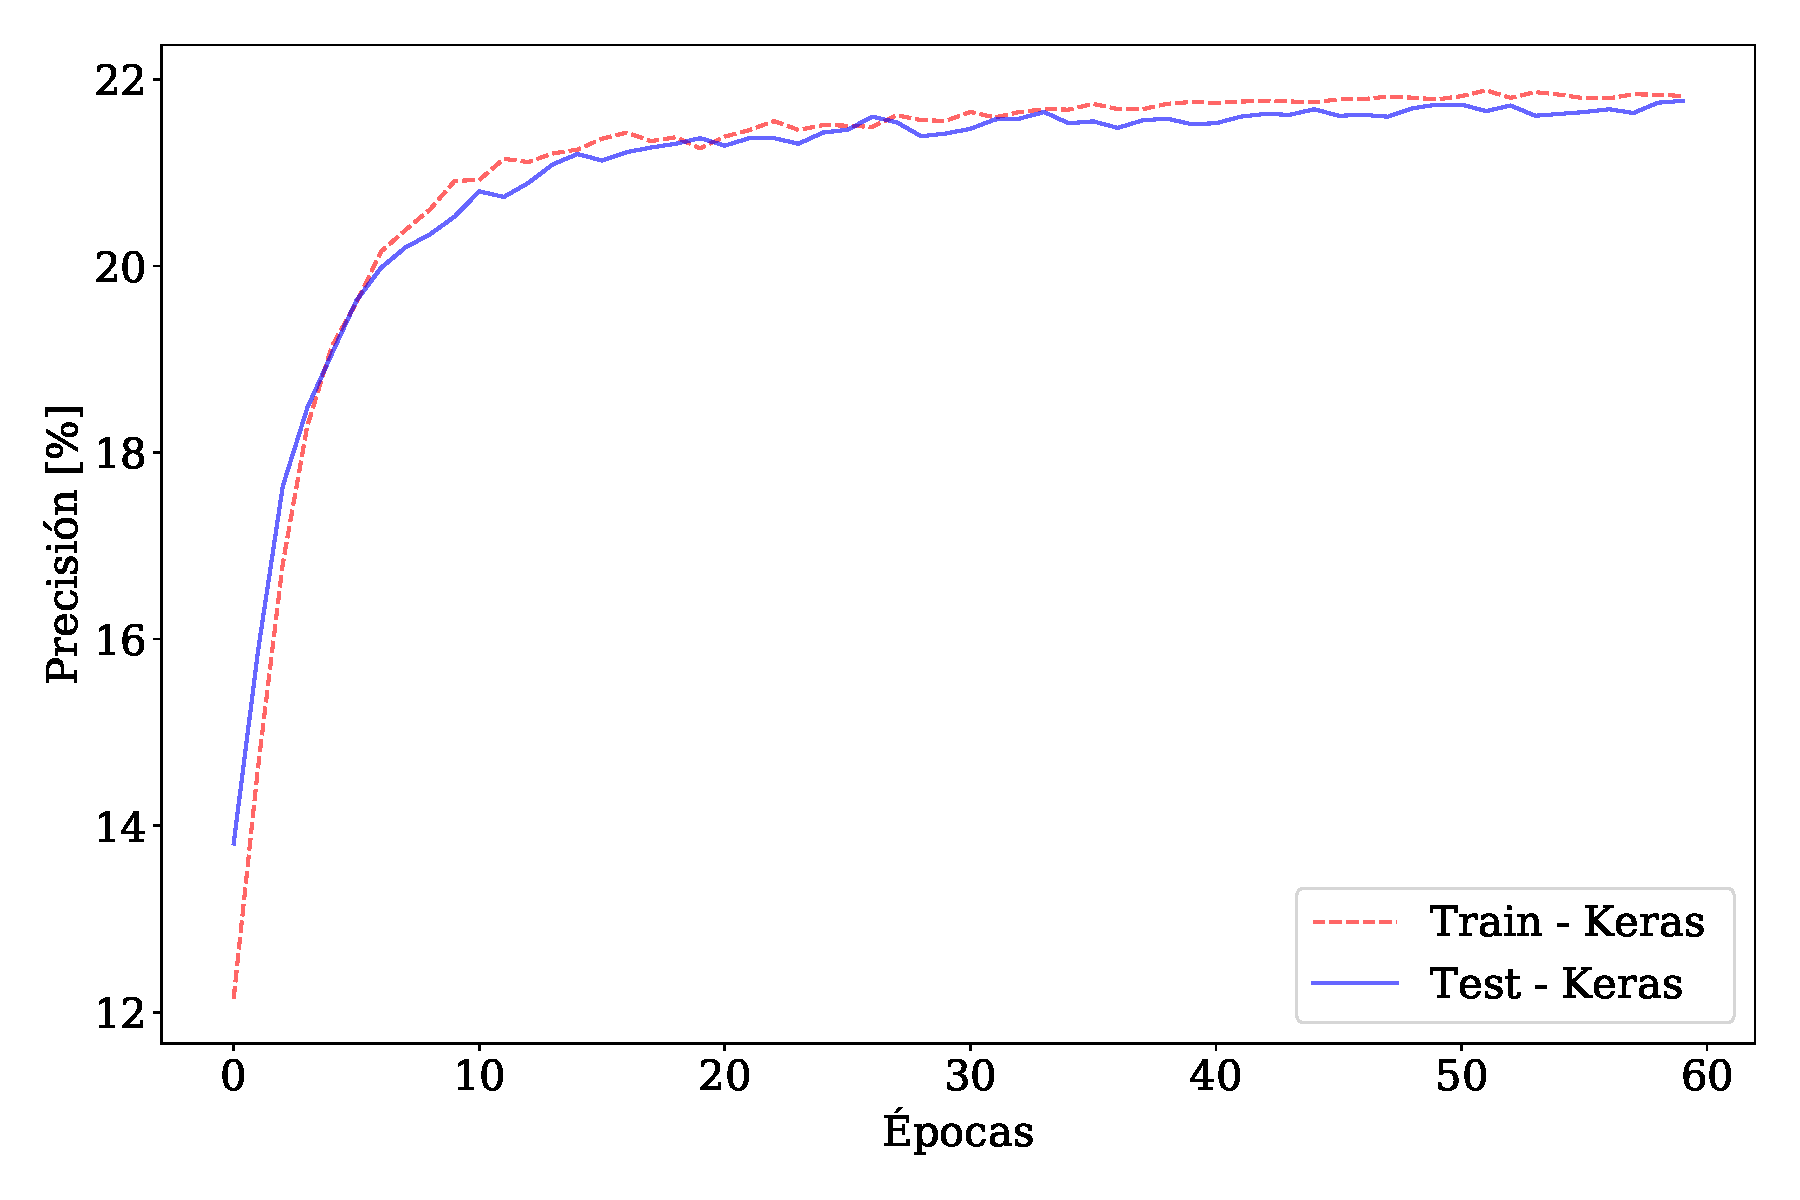
\includegraphics[width=0.5\textwidth]{Figs/ejer3_acc.pdf}
            \end{center}
            \caption{Precisión en función de las épocas}
            \label{fig:ejer3_acc}
        \end{small}
    \end{figure}
    En segunda instancia, con los mismos parámetros del primer entrenamiento se inicializaron los pesos de la red convolucional ya entrenados con \emph{imagenet}. En las figuras anteriores, estas curvas se identifican con \emph{Imag.}, se observa además que la red alcanza una mejor precisión  que el caso anterior como era de esperarse, donde la red empieza con una precisión alta del $38\%$ y llega al orden del $78\%$ de precisión. Las redes convolucionales con los pesos ya entrenados tiene la facilidad de reconocer los features propios de imágenes naturales.  


    Por último se entrenó la red usando \emph{Fine-tuning}. En este trabajo, este proceso consistió en entrenar las últimas dos capas de la red durante 20 épocas con las mismas condiciones que los casos anteriores, luego se permite a la red en modificar los pesos de las capas convolucionales durante 40 épocas con una tasa de aprendizaje de $10^{-5}$.  En las Figs.\ref{fig:ejer3_acc} y \ref{fig:ejer3_loss} las curvas que corresponden a este caso se identifican con \emph{FT}. Este trabajo esperaba que con los pesos ya entrenados la red alcanzaría una mejor precisión superior al primer caso, pero se observó que no sucedió en el caso de la curva de validación, esto puede deberse a que los features que aprendió la red clasificando \emph{imagenet} en 1000 categorías confunde a las últimas capas que buscan una clasificación de solamente 10.  Una vez que la red puede modificar  los pesos de las capas convolucionales, la precisión a partir de la época 40 aumenta considerablemente y llega a la misma precisión que el segundo caso. 


    \begin{figure}[H]
        \begin{small}
            \begin{center}
                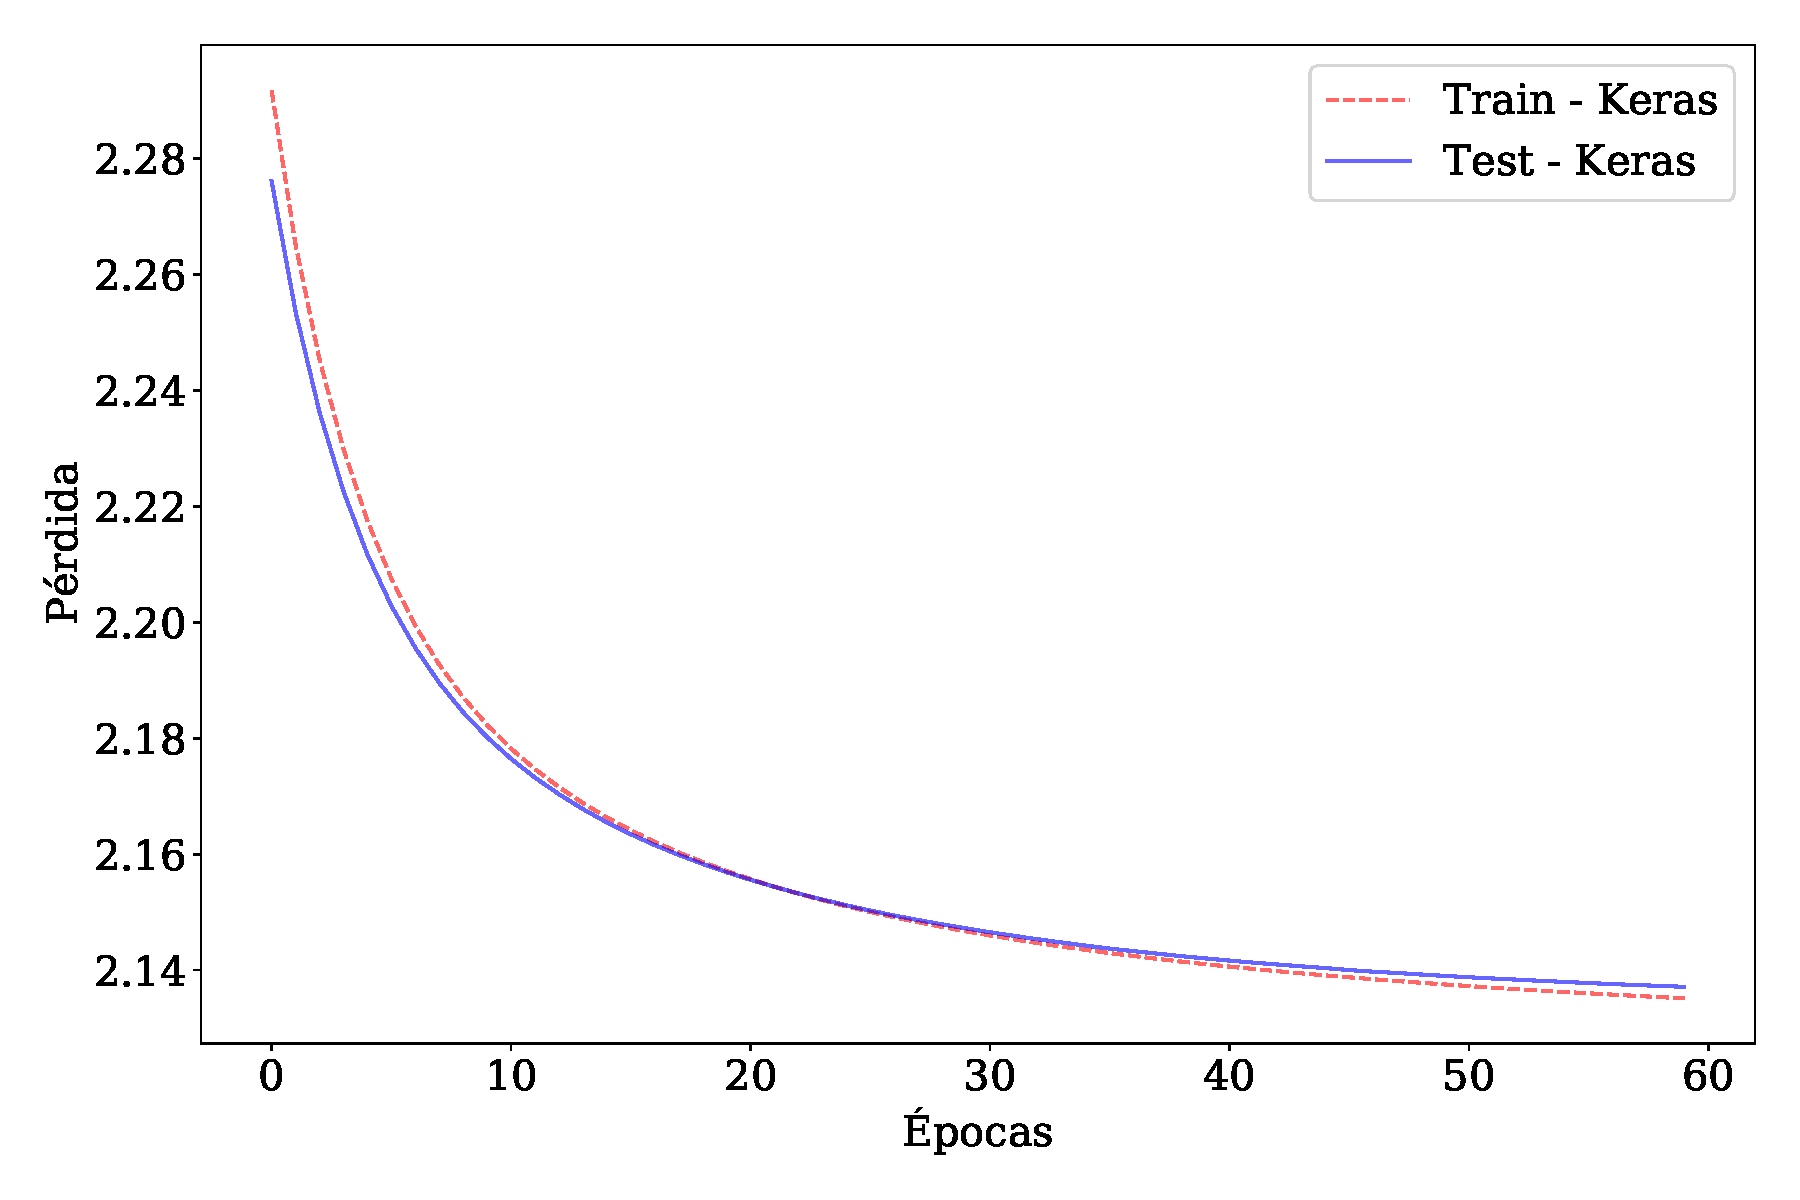
\includegraphics[width=0.5\textwidth]{Figs/ejer3_loss.pdf}
            \end{center}
            \caption{Pérdida en función de las épocas}
            \label{fig:ejer3_loss}
        \end{small}
    \end{figure}

    Este ejemplo de clasificar las imágenes del CIFAR-10 alcanza una  precisión alta dado que la red está entrenada en reconocer features en imágenes naturales. Si utilizáramos una red pre-entrenada en reconocer features en lenguaje natural u otro conjunto de datos, la red tendría una precisión pobre en la misma cantidad de épocas con respecto a la utilizada en este ejercicio.


\section*{Ejercicio 4}

Siguiendo con la red utilizada en el ejercicio anterior, ahora se busca visualizar lo que la red va analizando durante las capas convolucionales. En particular, nos centramos en lo que se observa en las antepenúltima y penúltima capa convolucional.

Para lograr esto se alimentó la red con tres tipos de imágenes: una imagen con píxeles de intensidad aleatoria que se muestra en la Fig.\ref{fig:random_init}, otra con píxeles que sigue un patrón sinusoidal como la Fig.\ref{fig:sin_init} por último una imagen natural, en este caso el perro de la Fig.\ref{fig:perro_init}. Las imágenes de los que se observa en las capas convolucionales son las Figs. \ref{fig:random_filters}, \ref{fig:sin_filters} y \ref{fig:perro_filters} respectivamente,  las imágenes de la izquierda y derecha corresponden a la antepenúltima y última capa.

Para realizar este ejercicio, este trabajo se basó en el ejemplo implementado por F. Chollet que se encuentra en la página de Keras \cite{keras}.

Primeramente se instancia un red que tenga como entrada la misma que la red \verb|MobileNet| y que tenga como salida la penúltima capa de la misma red. Una vez elegida las dimensiones de las imágenes de entrada, se aplica un algoritmo similar al gradiente descendente donde ahora se intenta maximizar la función de costo. La función de costo en este problema es la media entre la imagen de entrada y la imagen de salida en cada capa.

El algoritmo de gradiente ascendente se realiza con una tasa de aprendizaje de $10$ que está por encima de las utilizadas usualmente, y se maximiza la función de pérdida durante 50 épocas. Para obtener las Figs. \ref{fig:random_filters}, \ref{fig:sin_filters} y \ref{fig:perro_filters} se realiza el proceso inverso al preprocesado y se transforman las imágenes a RGB.

Con la imagen  aleatoria de la Fig.\ref{fig:random_init} se obtiene la Fig.\ref{fig:random_filters}, donde se observan  patrones en la parte del centro de la imagen, esto puede deberse a que la mayor parte de la información de las imágenes se encuentran en esta área. 

\begin{figure}[H]
    \begin{small}
        \begin{center}
            
\includegraphics[width=0.25\textwidth]{Figs/random_init_img_epochs_50.pdf}
        \end{center}
        \caption{Imagen con valores aleatorios en los tres canales RGB.}
        \label{fig:random_init}
    \end{small}
\end{figure}


\begin{figure}[H]
    \begin{small}
        \begin{center}
            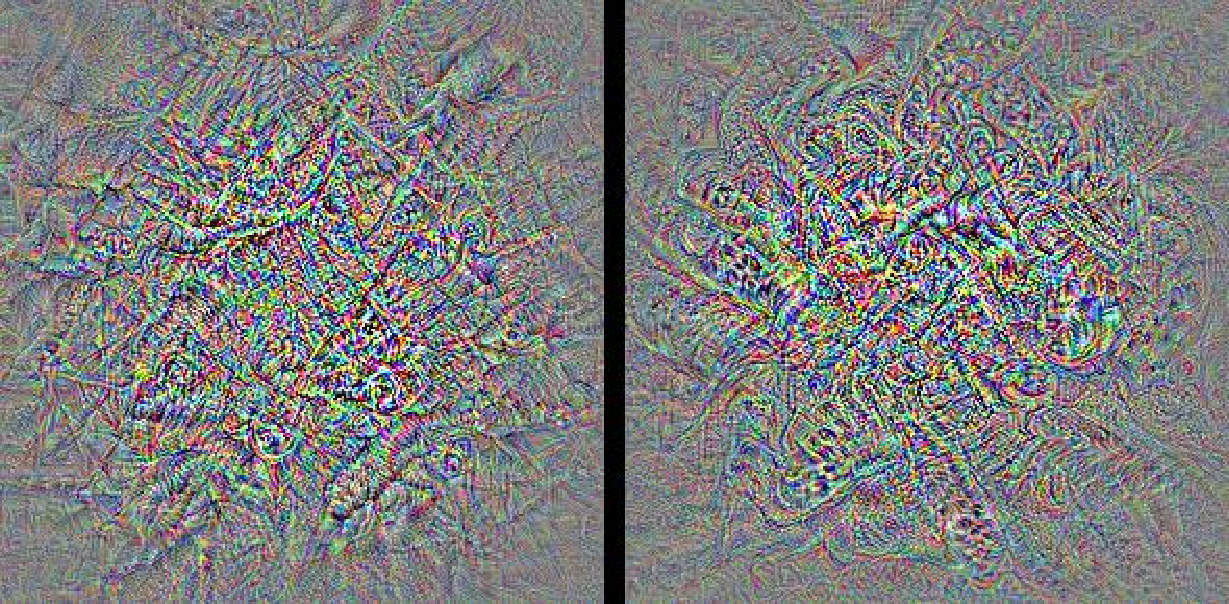
\includegraphics[width=0.5\textwidth]{Figs/random_filters_epochs_50.pdf}
        \end{center}
        \caption{Imágenes obtenidas mediante el gradiente ascendente a a partir de la imagen aleatoria.}
        \label{fig:random_filters}
    \end{small}
\end{figure}

Con la imagen  con patrón sinusoidal de la Fig.\ref{fig:sin_init} se obtiene la Fig.\ref{fig:sin_filters}, donde además de observarse los  patrones en la parte del centro de la imagen, la red intenta obtener información sobre las líneas de la imagen original. Este es el proceso por el cual la red convolucional intenta reconocer features en las imágenes. 

\begin{figure}[H]
    \begin{small}
        \begin{center}
            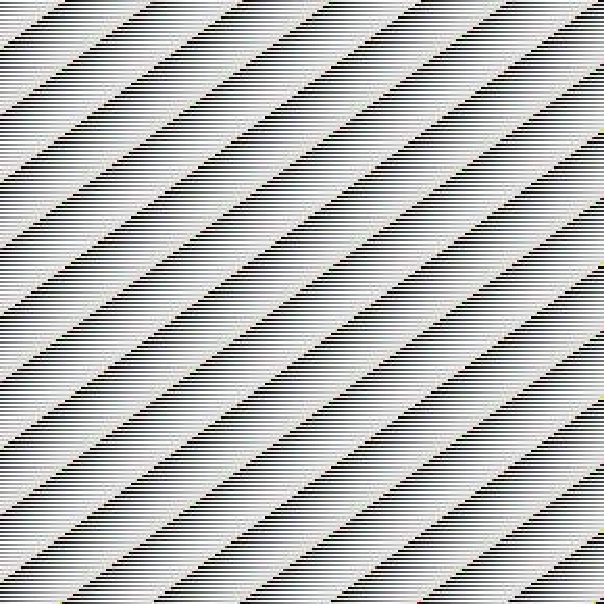
\includegraphics[width=0.25\textwidth]{Figs/sin_init_img_epochs_50.pdf}
        \end{center}
        \caption{Imagen con un patrón sinusoidal en las componentes RGB.}
        \label{fig:sin_init}
    \end{small}
\end{figure}

\begin{figure}[H]
    \begin{small}
        \begin{center}
            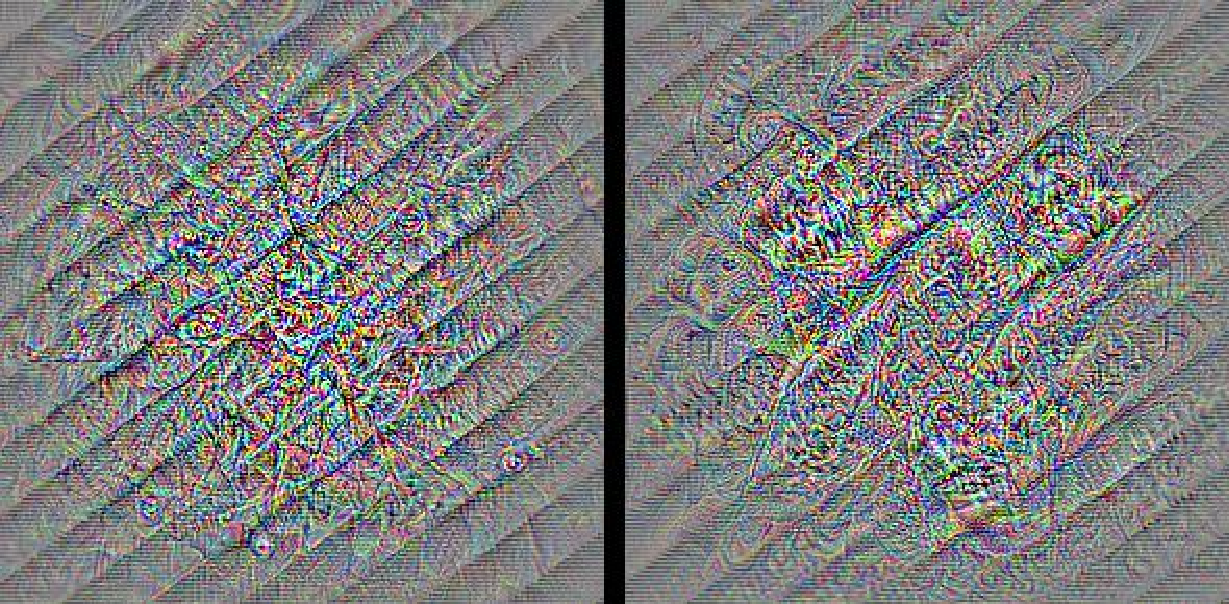
\includegraphics[width=0.5\textwidth]{Figs/sin_filters_epochs_50.pdf}
        \end{center}
        \caption{Imágenes obtenidas mediante el gradiente ascendente a a partir de la imagen con el patrón sinusoidal.}
        \label{fig:sin_filters}
    \end{small}
\end{figure}

Con la imagen  del animal de la Fig.\ref{fig:perro_init} se obtiene la Fig.\ref{fig:perro_filters}. Esta imagen de entrada es un ejemplo de como la red intenta obtener información sobre el outline sobre la parte  central de la imagen original. Por ejemplo, en este caso la red omite información del fondo del animal, esto es posible después del entrenamiento de las capas.



\begin{figure}[H]
    \begin{small}
        \begin{center}
            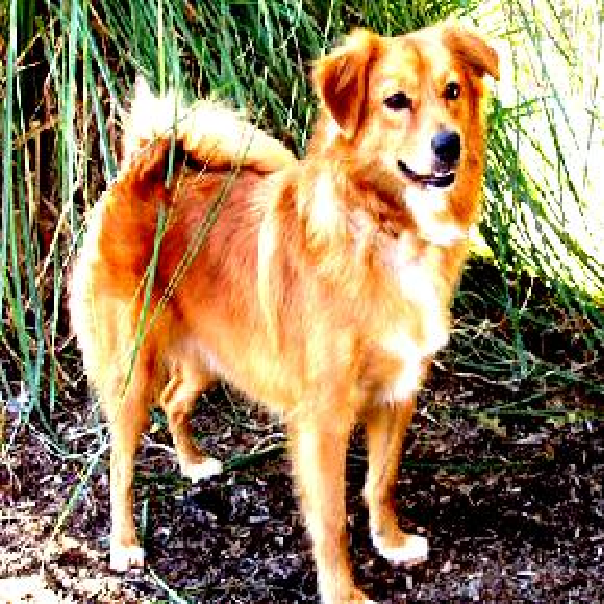
\includegraphics[width=0.25\textwidth]{Figs/perr2_init_img_epochs_50.pdf}
        \end{center}
        \caption{Imagen de un perro del conjunto de datos dogs vs cats.}
        \label{fig:perro_init}
    \end{small}
\end{figure}

\vfill\null


\begin{figure}[H]
    \begin{small}
        \begin{center}
            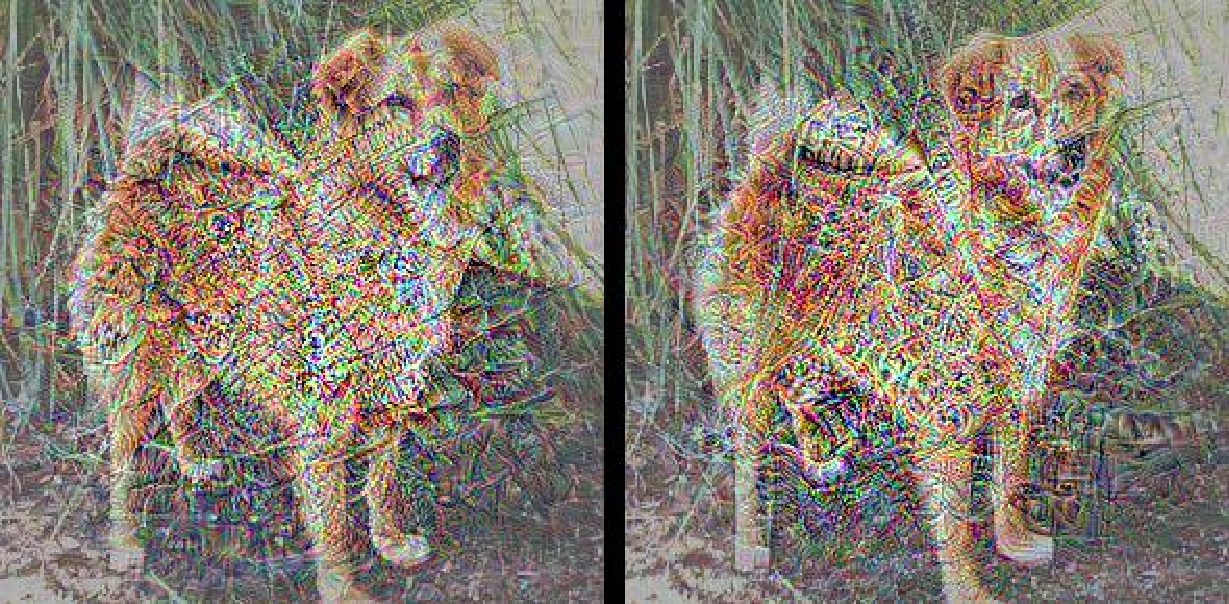
\includegraphics[width=0.5\textwidth]{Figs/perr2_filters_epochs_50.pdf}
        \end{center}
        \caption{Imágenes obtenidas mediante el gradiente ascendente a a partir de la imagen de un perro.}
        \label{fig:perro_filters}
    \end{small}
\end{figure}


\bibliographystyle{apsrev4-1}
\bibliography{mibib.bib}


\end{document}